\documentclass[12pt, a4paper]{article}
\usepackage{amsmath, amssymb, amsfonts} 
\usepackage{inputenc}
\usepackage{float}
\usepackage{graphics}                 
\usepackage{color}                    
\usepackage{hyperref}
\usepackage{ptext}
\usepackage{graphicx}   
%\usepackage[export]{adjustbox}                     
%\settextfont[Scale=.9]{Calibri}

%\graphicspath{ {images/} }

\hypersetup{
	colorlinks=true,
	linkcolor=blue,
	filecolor=magenta,      
	urlcolor=cyan
}


\title{
	{\Huge \textbf{In the name of God}}
	\\[20pt]
	
\includegraphics[width=0.5\linewidth]{../assets/IUST_logo_color_eng.jpg} \\
	{\normalsize Department of Computer Engineering}
}

\author{
	\\[10pt]
	\textbf{{\LARGE Natural Language Processing}}
	\\[10pt]
	\LARGE Final Phase Report
	\thanks{\url{https://github.com/yegmor/NLPProject}}
	
	\\[30pt]
	\textbf{Yeganeh Morshedzadeh}
	\\[5pt]
	Student Number: 96521488
}

\date{Spring 2021} 

\begin{document}
	
	\maketitle
	%\graphicspath{{../reports/images}}‎
	
	\clearpage
	%\addtocontents{toc}{\textbf{Content}~\hfill\textbf{Page}\par}
	\tableofcontents
	\newpage
	
	\listoffigures
	\newpage
	
	\listoftables
	\newpage
	
	\begin{abstract}
		In this project, we tried to use Natural Language Processing to better understand Depression and Anxiety posts. The dataset is gathered from Reddit communities \href{https://www.reddit.com/r/depression}{r/depression} and \href{https://www.reddit.com/r/Anxiety}{r/Anxiety}.
		\\[10pt]
		
		For this project, at first, we wrote a project proposal (\href{https://docs.google.com/document/d/1tHGEmEgn8-sp8MD72d8NjnZsq-GpVupzsMWgnqaGi-Y/edit?usp=sharing}{Google Docs}), and afterward, in the first phase (\href{https://docs.google.com/document/d/1Jc2ELhweU01Tbf0WalU7wVQABdAV4w50mhQnmMpU2mM/edit?usp=sharing}{Google Docs}), we gathered data and made some exploratory data analysis. 
		\\[10pt]
		
		In the final phase, we went deeper and tried various NLP tasks, such as, computing Word2Vec, Tokenization, Parsing, and creating a language model based on our dataset.
	\end{abstract}
	
	\newpage
	\part{Word2Vec}
	\large{\textbf{Filename:} 3\_word2vec.ipynb}
	\section{Overview}
	
	\subsection{Code}
	We used \href{https://radimrehurek.com/gensim/models/word2vec.html}{Gensim implementation of word2vec}. 
	
	For this part, we have three Word2Vec models, named dep\_w2v\_model, anx\_w2v\_model, and all\_w2v\_model. Moreover, with boolean parameters, load and save, the model will be saved and/or loaded in the my\_word2vec function.
	
	\begin{table}[H]
		\caption{Word2Vec vocabulary size} 
		\centering 
		\vspace{5mm} 
		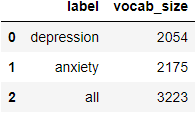
\includegraphics[width=0.5\linewidth]{../reports/images/w2v_vocab-size.png}
		\label{w2v_vocab-size} 
	\end{table}
	
	
	\subsection{Results and Examples}
	In this part, we used t-SNE visualization. t-SNE is a non-linear dimensionality reduction algorithm that attempts to represent high-dimensional data and the underlying relationships between vectors in a lower-dimensional space.
	
	To make the visualizations more relevant, we will look at the relationships between a query word (in \textcolor{red}{**red**}), its most similar words in the model (in \textcolor{blue}{**blue**}), and other words from the vocabulary (in \textcolor{green}{**green**}).
	\begin{figure}[H]
		\centering{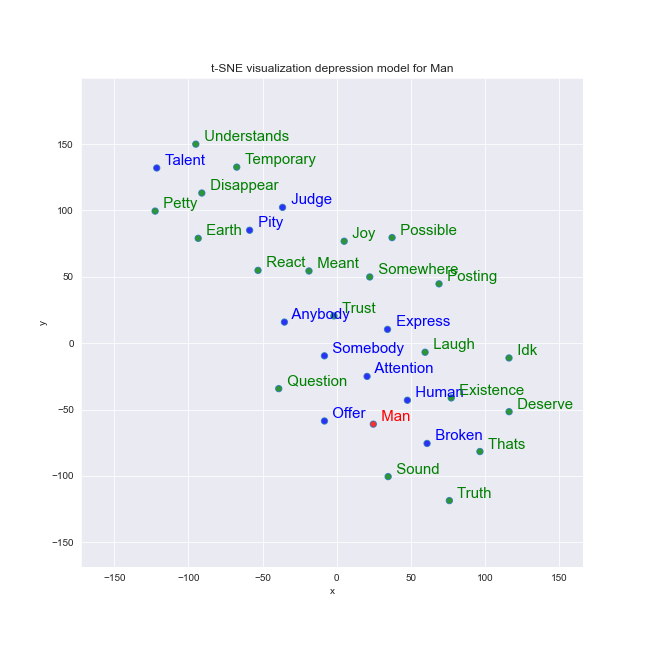
\includegraphics[width=\linewidth, height=\textheight, keepaspectratio]{../reports/images/word2vec_depression_man.png}}
		\caption{t-SNE visualization for man}
		\label{word2vec_depression_man}
	\end{figure}
	
	\newpage
	\part{Tokenization}
	\large{\textbf{Filename:} 4\_tokenization.ipynb}
	\section{Overview}
	
	\subsection{Code}
	In this part, we have used KFold to split(=5) our data into train and test. Afterward, we train the SentencePiece model based on the data. Lastly, we evaluate the model by computing <UNK> on our test dataset and finally choosing as well as hard coding the best model for the tokenizer. 
	
	\subsection{Results and Examples}
	Based on Table \ref{token_vocab-size}, in which the percentage of unk tokens to all tokens is calculated for each vocabulary size, we can conclude that by setting higher vocabulary size for the tokenizer, the number of <UNK>s decreases.
	
	Therefore, the best tokenizer is the one with a larger vocabulary size (=9000).
	
	\begin{table}[H]
		\caption{Tokenizer outcome based on different vocabulary sizes} 
		\centering 
		\vspace{5mm} 
		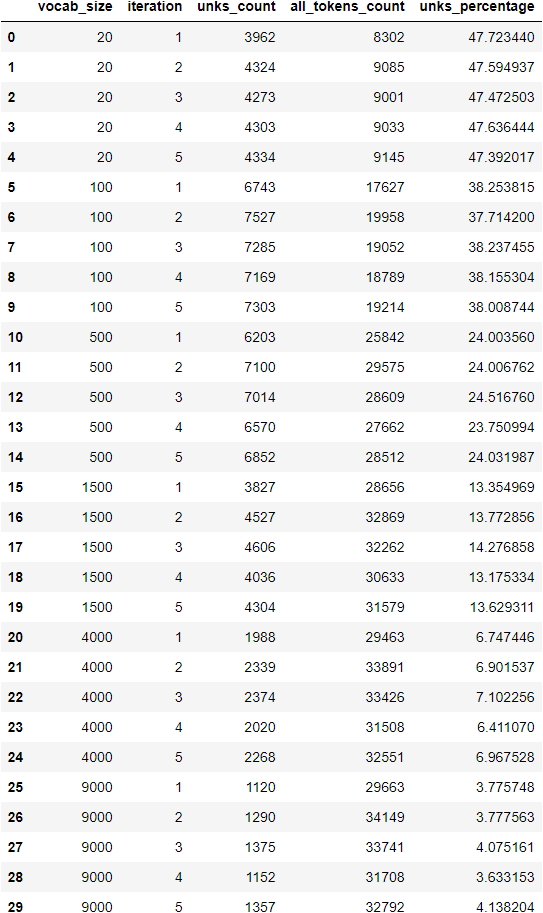
\includegraphics[width=\linewidth, height=\textheight]{../reports/images/token_vocab-size.png}
		\label{token_vocab-size} 
	\end{table}
	
	
	
	\newpage
	\part{Parsing}
	\large{\textbf{Filename:} 8\_parsing}
	\section{Overview}
	In this part, we used Stanza, which is a Python NLP Package, and a collection of accurate and efficient tools for the linguistic analysis of many human languages. Starting from raw text to syntactic analysis and entity recognition, Stanza brings state-of-the-art NLP models to languages of your choosing.
	
	More specifically, we used their \href{http://stanza.run/}{Online Demo} to create a manual CoNLL file based on our dataset (my\_test.conll). Later, we can use \href{https://universaldependencies.org/conllu_viewer.html}{Universal Dependencies CoNLL viewer} to automatically generate parse tree from CoNLL file.
	
	\subsection{Results and Examples}
	We chose 10 sentences from our dataset as shown below.
	\begin{enumerate}
		\item I never really showed any sadness when I am with someone.
		\item he is a good person, and I know that.
		\item how am I feeling?
		\item last year I went through a huge amount of stress.
		\item how can you tell the difference between an actual issue or anxiety?
		\item please do not judge.
		\item what do you think is the meaning of life?
		\item today was a very strange day.
		\item all these emotions are too much sometimes. 
		\item everybody is going to die.
	\end{enumerate}
	
	Afterwards, we created a CoNLL file as shown in Figure \ref{parsing_conll}. 
	\begin{figure}[H]
		\centering{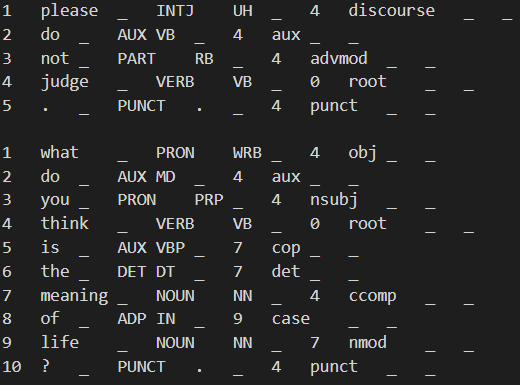
\includegraphics[width=\linewidth, height=\textheight, keepaspectratio]{../reports/images/parsing_conll.png}}
		\caption{conll format of 6th and 7th sentences}
		\label{parsing_conll}
	\end{figure}
	
	For creating the .conll we used Stanza visualization to help us understand Universal Dependencies. (Figure \ref{parsing_examples_UDtree})
	\begin{figure}[H]
		\centering{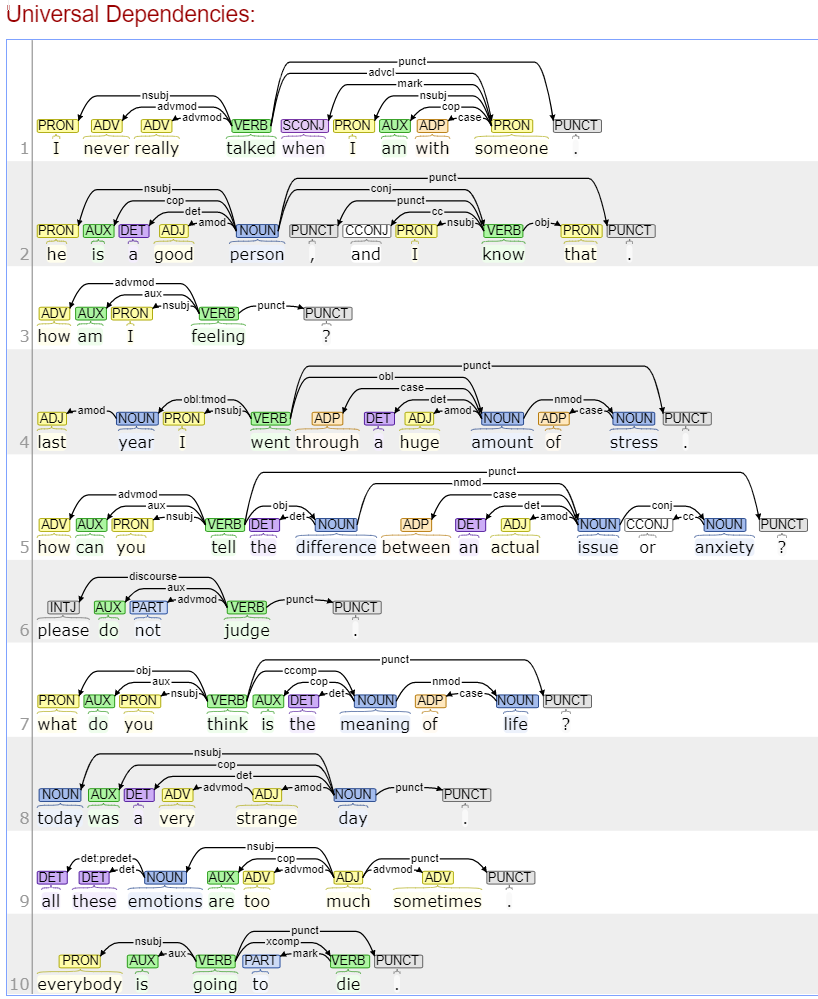
\includegraphics[width=\linewidth, height=\textheight, keepaspectratio]{../reports/images/parsing_examples_UDtree.png}}
		\caption{Universal Dependencies for 10 sentences}
		\label{parsing_examples_UDtree}
	\end{figure}
	
	The reported Unlabeled Attachment Score (UAS) on our test file was 94.19, and the output of the code for dependencies are show in Figure \ref{parsing_output}. 
	\begin{figure}[H]
		\centering{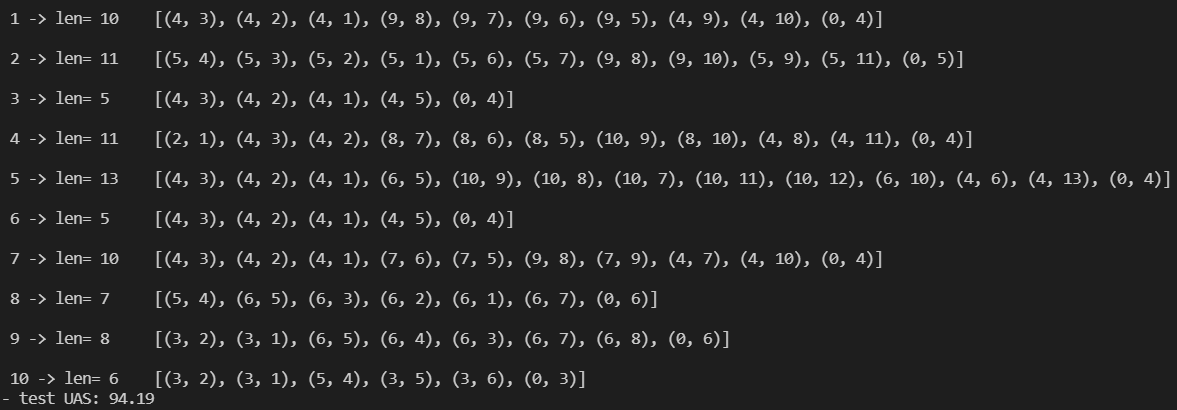
\includegraphics[width=\linewidth, height=0.4\textheight, ]{../reports/images/parsing_output.png}}
		\caption{Outputs for the my\_test.conll}
		\label{parsing_output}
	\end{figure}
	
	When comparing Figure \ref{parsing_examples_UDtree} and Figure \ref{parsing_output}, we can see couple of mistakes:
	\begin{itemize}
		\item \textbf{Sentence no.2}: \emph{he is a good person, and I know that.}
		
		The parent of \emph{and}, \emph{person}, and \emph{,} should be \emph{know}, and that \emph{know} is the root. However, our model thinks\emph{person} is the root.
		
		\item \textbf{Sentence no.5}:
		\emph{how can you tell the difference between an actual issue or anxiety?}
		
		The parent of \emph{or} should be \emph{anxiety}, whereas our model thinks it is \emph{issue}.
	\end{itemize}
	
	Therefore, it looks like that the model in some cases fails to completely understand dependencies in complex sentences. 
	
	\newpage
	\part{Language Model}
	\large{\textbf{Filename:} 5\_language-model.ipynb}
	\section{Overview}
	In this part, we have developed a model of the text that we can then use to generate new sequences of text. It is worth noting that we have used \emph{selftext\_clean} column of our data frame to train this model.
	
	\subsection{Code}
	We will start by preparing the data for modeling. 
	We have picked a length of 50 words for the length of the input sequences, and we have attached 1 output word at the end of the sequences. Afterward, we save the long list of sequences.
	
	For our language model, after loading our dataset, we used an Embedding Layer to learn the representation of words, and a Long Short-Term Memory (LSTM) recurrent neural network to learn to predict words based on their context. More precisely, we have used two LSTM hidden layers with 100 memory cells each. Following, we have a dense fully connected layer with 100 neurons connects to the LSTM hidden layers to interpret the features extracted from the sequence. The summary of the model is shown in Figure \ref{normal-lm_arch}.
	
	After the model is trained, we use generate\_seq function that takes as input the model, the tokenizer, input sequence length, the seed text, and the number of words to generate. 
	
	Moreover, with boolean parameters, load\_bool and save, the specific model will be saved and/or loaded.
	\begin{figure}[H]
		\centering{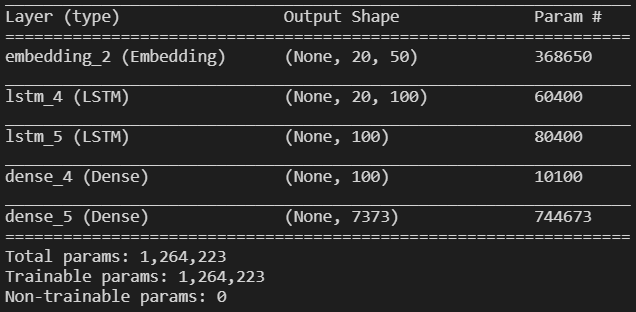
\includegraphics[width=\linewidth, height=\textheight, keepaspectratio]{../reports/images/normal-lm_arch.png}}
		\caption{Model architecture for simple language model}
		\label{normal-lm_arch}
	\end{figure}
	
	\subsection{Results and Examples}
	Since we have used the \emph{selftext\_clean} column of our data and therefore the stopwords, as well as punctuation symbols, are removed, we see that our model can not follow grammatical rules and make complete sentences. 
	\\In addition, as we have not used pre-train models, the model requires more data to generate better sentences. 
	
	Overall, the model was somehow not bad at capturing the context of the dataset. 
	
	In Table \ref{normal-lm_examples}, by feeding the seed text, obtained randomly from either depression or anxiety dataset, the model generates a sequence.
	\begin{table}[H]
		\caption{Examples for simple language model} 
		\centering 
		\vspace{5mm} 
		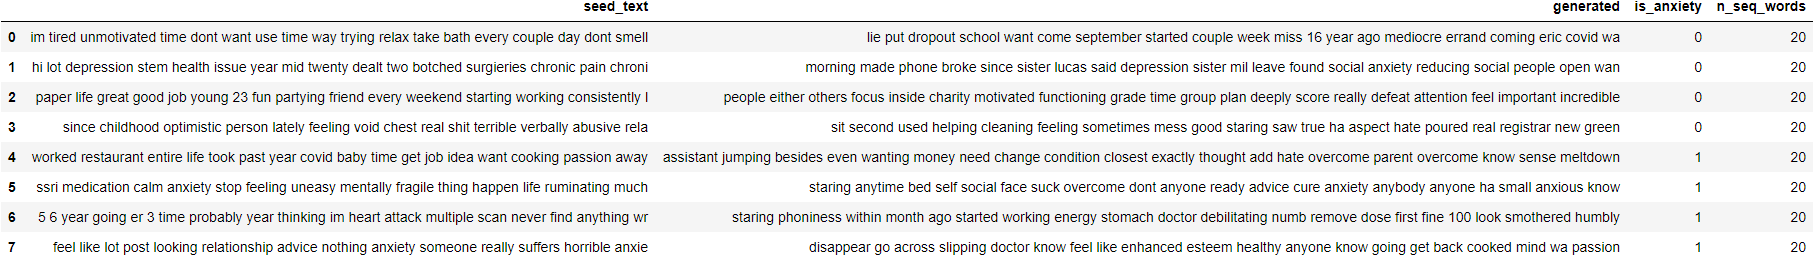
\includegraphics[width=1.2\linewidth, 
		keepaspectratio]{../reports/images/normal-lm_examples.png}
		\label{normal-lm_examples} 
	\end{table}
	
	\newpage
	\part{Fine-tuning}
	\section{Classification}
	\large{\textbf{Filename:} 6\_finetune\_classification.ipynb}
	
	Since some files exceeded GitHub's maximum file size (100Mb), we have uploaded them in Google drive.
	\begin{itemize}
		\item \href{https://drive.google.com/file/d/1Lbbhh2N92k3IjuZ5TObauPd2en5qAT6i/view?usp=sharing}{bert\_classification\_lm-pytorch\_model.bin}
	\end{itemize}
	
	In this part, we have trained three distinct models, two of which are used to generate a model with respect to the label (depression or anxiety), and one model is used to classify the text into two categories (depression and anxiety).
	
	\subsection{Code}
	For classification, we used the pre-trained \emph{google/bert\_uncased\_L-4\_H-512\_A-8} model. We then tokezie, truncate, and pad our dataset to a specific length (=max\_length), and create a torch dataset out of them.
	
	We used Trainer API to train our model. The Hyperparameters that are being used are set in the TrainingArguments.
	
	\begin{table}[H]
		\caption{Training bert classification language model}
		\centering
		\vspace{5mm} 
		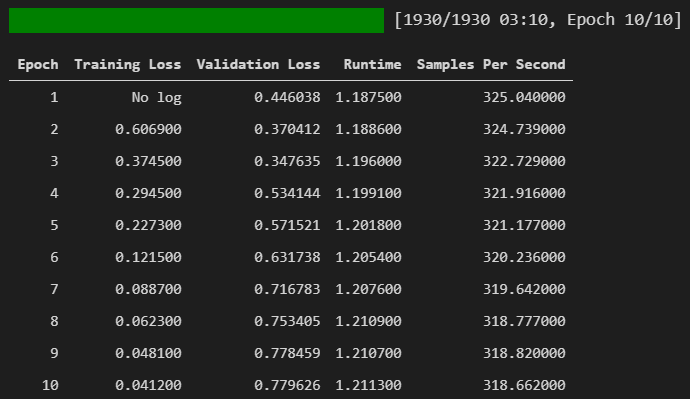
\includegraphics[width=\linewidth, height=\textheight, keepaspectratio]{../reports/images/classification-lm_train.png}
		\label{classification-lm_train}
	\end{table}
	
	
	\subsection{Results and Examples}
	As shown in Figure \ref{classification-lm_eval} , the accuracy of the model on the validation dataset is 87.30\%.
	
	\begin{figure}[H]
		\centering{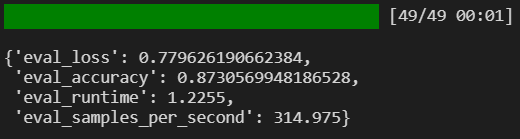
\includegraphics[width=\linewidth, height=\textheight, keepaspectratio]{../reports/images/classification-lm_eval.png}}
		\caption{Evaluating bert classification language model}
		\label{classification-lm_eval}
	\end{figure}
	
	We also selected some sentences from the dataset randomly and fed them to the model to see how it does. The results are shown in Table \ref{classification-lm_examples}.
	
	\begin{table}[H]
		\caption{Examples for bert classification model}
		\centering
		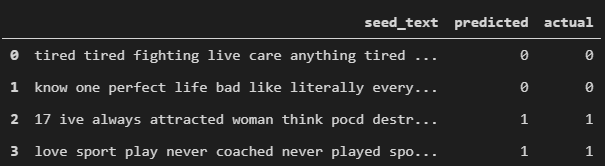
\includegraphics[width=\linewidth, height=\textheight, keepaspectratio]{../reports/images/classification-lm_examples.png}
		\label{classification-lm_examples}
	\end{table}
	
	
	\section{Language Model}
	\large{\textbf{Filename:} 7\_finetune\_language-model.ipynb}
	
	Since some files exceeded GitHub's maximum file size (100Mb), we have uploaded them in Google drive. 
	\begin{itemize}
		\item \href{https://drive.google.com/file/d/1AmbAl9mFoGG9mITTTz7TRgPEwVUAiN9U/view?usp=sharing}{depression.bert\_lm-pytorch\_model.bin}
		\item
		\href{https://drive.google.com/file/d/19-KhVSsBFo7WpfzeXNKDpUnYKv5xfDkY/view?usp=sharing}{anxiety.bert\_lm-pytorch\_model.bin}
	\end{itemize}
	
	\vspace{5mm}
	In this part, we have used our Reddit dataset to fine-tune our distilgpt-2.
	
	For this purpose, we first prepare the dataset and build a TextDataset, load the pre-trained GPT-2 model and tokenizer, initialize Trainer with TrainingArguments, and finally, train and save the model. 
	
	\subsection{Code}
	The TextDataset is a custom implementation of the Pytroch Dataset class implemented by the transformers(4.2.2) library.
	\\Also, we have used the tokenizer from the distilgpt-2 model on huggingface.
	\\Afterwards, we initialize the Trainer class that provides an API for feature-complete training, and we set the Hyperparameters we are going to use in the TrainingArguments.
	
	\subsection{Results and Examples}
	This section is quite the same as the section in the previous part (Language Model). 
	
	Similar to that part we have used the \emph{selftext\_clean} column of our data and therefore the stopwords, as well as punctuation symbols, are removed, we see that our model can not follow grammatical rules and use pronouns. The difference is that we have used a far better and more powerful model to do our language modeling task.
	
	The model does pretty well at producing sentences similar to the context of the sentence considering the label (depression or anxiety). In other words, the quality of the generated text is high, and the sentence is much more meaningful. 
	
	Moreover, as shown in Table \ref{finetune-lm_examples}, the difference between the generated sentences for the same seed text is more distinguishable and really fits the context of each label.
	
	\begin{table}[H]
		\caption{Examples for distilgpt2 language model}
		\centering
		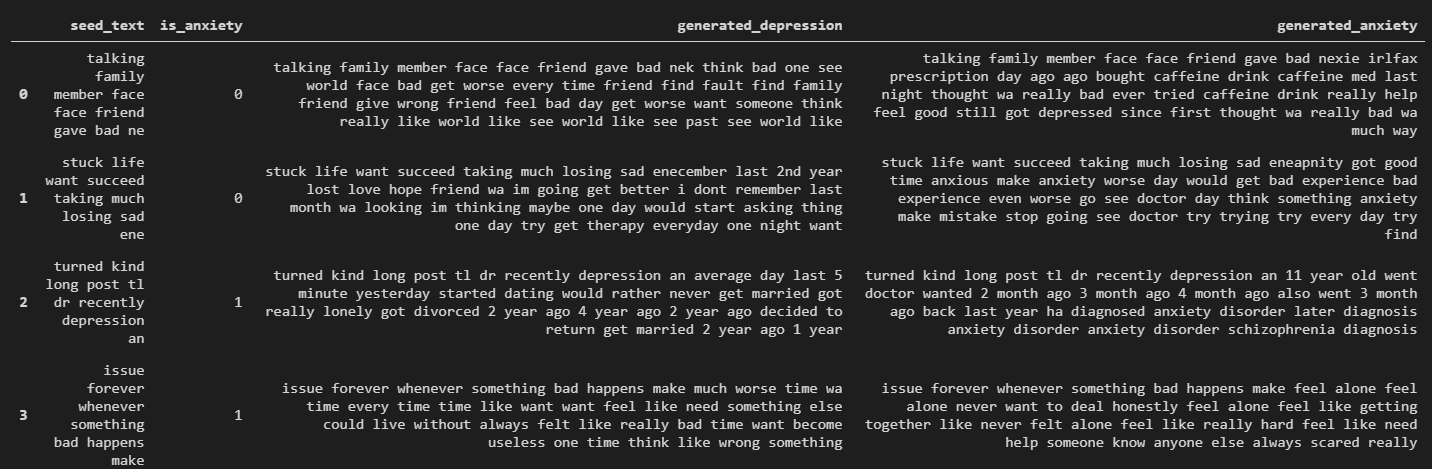
\includegraphics[width=\linewidth, height=0.3\textheight]{../reports/images/finetune-lm_examples.png}	
		\label{finetune-lm_examples}
	\end{table}
	
	
	\newpage
	\begin{thebibliography}{9}
		\bibitem{bib0}
		\url{https://towardsdatascience.com/goodbye-world-4cc844197d51}
		
		\bibitem{bib1}
		\url{https://colab.research.google.com/github/google/sentencepiece/blob/master/python/sentencepiece_python_module_example.ipynb#scrollTo=ee9W6wGnVteW}
		
		\bibitem{bib2}
		\url{https://gmihaila.github.io/tutorial_notebooks/gpt2_finetune_classification/}
		
		\bibitem{bib3}
		\url{https://colab.research.google.com/github/philschmid/fine-tune-GPT-2/blob/master/Fine_tune_a_non_English_GPT_2_Model_with_Huggingface.ipynb}
		
		\bibitem{bib4}
		\url{https://github.com/huggingface/notebooks/blob/master/examples/language_modeling.ipynb}
		
		\bibitem{bib5}
		\url{https://www.kaggle.com/pierremegret/gensim-word2vec-tutorial}
		
		\bibitem{bib6}
		\url{https://machinelearningmastery.com/how-to-develop-a-word-level-neural-language-model-in-keras/}
		
		\bibitem{bib7}
		\url{https://huggingface.co/transformers/training.html}
		
		\bibitem{bib8}
		\url{https://www.kaggle.com/achintyatripathi/gensim-word2vec-usage-with-t-sne-plot}
		
		\bibitem{bib9}
		\url{https://colab.research.google.com/github/borisdayma/huggingtweets/blob/master/huggingtweets-demo.ipynb}
		
		\bibitem{bib10}
		\url{https://huggingface.co/transformers/custom_datasets.html}
		
		\bibitem{bib11}
		\url{https://colab.research.google.com/github/google/sentencepiece/blob/master/python/sentencepiece_python_module_example.ipynb#scrollTo=-k5KbVgiYae-}
		
		\bibitem{bib12}
		\url{https://colab.research.google.com/drive/1ZZ9vJ_nIQkgjW776lnPvwVfRHuOKvbz8}
		
	\end{thebibliography}
	
\end{document}          
